% Intended LaTeX compiler: pdflatex
\documentclass[koma,utopia,a4paper,captions=tableheading,11pt,listings-sv,microtype,paralist,colorlinks=true,urlcolor=blue]{org-article}
               \usepackage{tikz}
\author{Eason}
\date{\today}
\title{Drawing Graphs Using TikZ in Emacs Org}
\hypersetup{
 pdfauthor={Eason},
 pdftitle={Drawing Graphs Using TikZ in Emacs Org},
 pdfkeywords={},
 pdfsubject={This post collects working examples of drawing graphs using TikZ in Emacs Org},
 pdfcreator={Emacs 26.3 (Org mode 9.2.6)},
 pdflang={English}}
\begin{document}

\newcommand*{\titleCM}{\begingroup
\vspace*{\drop}
\begin{center}
\vspace{\baselineskip}
{\Huge \textbf{Drawing Graphs Using TikZ in Emacs Org} \par}
\vspace{2\baselineskip}   \newline
{\large Eason Zhang with www.makesteamclear.com \par}
\vspace{\baselineskip}          \newline
{\large \today \par}
\vspace{\baselineskip}
\vfill
\setlength{\unitlength}{3pt}
\makebox[\textwidth][c]{\includegraphics[width=0.5\textwidth]{/Users/chaolongzhang/Dropbox/mstemc_hugo/static/img/tikz/example3.pdf}}
\vfill
\vspace{\baselineskip}
{\Large WWW.MAKESTEAMCLEAR.COM \par}\newline
\vspace{\baselineskip}
{\texttt www.makesteamclear.com is a free project, supported by Eason Zhang, to make videos about STEAM in a more approachable and different way. If you found the contents in this post or the site or the youtube channel helpful, please consider support me, thanks \par}
\end{center}
\vspace*{\drop}
\endgroup}
\begin{titlepage}
\titleCM
\end{titlepage}
\tableofcontents




\section{Drawing a TikZ picture in Emacs Org Mode}
\label{sec:org8d51a0b}


\lstset{language=[LaTeX]TeX,label=a-minimum-working-example,caption={a minimum working example},captionpos=b,firstnumber=1,numbers=left}
\begin{lstlisting}
\usetikzlibrary{intersections,arrows.meta}
\begin{tikzpicture}[thin]
\draw (-1.5,0) -- (1.5,0);
\draw (0,-1.5) -- (0,1.5);
\filldraw[fill = green!20, draw = green!50!black] (0,0) circle[radius = 1cm];
\draw (0,0) rectangle (.5,.5);
\draw (0,0) rectangle (-0.5,-0.5);
\draw[help lines,very thin,step=.5cm,color=gray] (-1.5,-1.5) grid (1.5,1.5);
% relative coordinate
\draw[blue, very thick] (30:1) ++ (0,-0.5) --(0,0);
% name a path without drawing it
\path[name path = upward line] (1,0) -- (1,1);
\path[name path = sloped line] (0,0) -- (30:1.5cm);
% use intersection of two path
\draw[name intersections={of = upward line and sloped line, by=x}]
     [very thick, orange] (1,0) -- (x);
% use arrow
\draw[<->>] (0,0) -- (145:1);
\draw[<-{Triangle[fill=red]}] (0,0) -- (30:1);
% use scope
\begin{scope}[very thick]
\draw (-0.4,0.4) -- (0.4,0.4);
\draw (-0.4,-0.4) -- (0.4,-0.4);
\end{scope}
% use foreach
\foreach \x in {-1cm,-0.5cm,1cm}
    \draw[red] (\x,-3pt) -- (\x,3pt);
\foreach \y in {-1cm,-0.5cm,1cm}
    \draw[red](-3pt,\y) -- (3pt,\y);
% using node
\draw (0,0)+(0.2,-0.2) node {\tiny $(0,0)$ };
\end{tikzpicture}
\end{lstlisting}


\hspace{0pt}\\
The generated figure is shown as:
\begin{center}
\includegraphics[width=0.5\textwidth]{/Users/chaolongzhang/Dropbox/mstemc_hugo/static/img/tikz/example3.pdf}
\end{center}

\begin{enumerate}
\item In \hyperref[a-minimum-working-example]{the minimum working example} line 12 , a path is named  without drawing
it.
\item Line 16 gives an example of using library \texttt{intersections}. Note
that you need to add the library using \texttt{\textbackslash{}usetikzlibrary\{intersections\}}
otherwise an error occurs during \LaTeX compiling.
\item Line 18 and 19 gives an example of using arrow. To make it work,
\texttt{\textbackslash{}usetikzlibrary\{arrows.meta\}} is needed. The library \texttt{arrows.meta} provides tons
of types of arrows whick shock me when I see them the first time.
\item Line 21 to 24 gives an example of \texttt{scope} . In the environment, all
the lines are drawn in the \texttt{very thick} style.
\item Line 26 to 29 gives an examplt of \texttt{foreach} . \texttt{foreach} is handy
when you want to draw a list of objects. In \hyperref[a-minimum-working-example]{the minimum working example} , I
draw a list of short red sticks along with the x-axis and y-axis.
\item Line 31 is an example of \texttt{node}. The keyword \texttt{node} is typically followed by
some options between \texttt{[]} and then some text between \texttt{\{\}}. Every node has flexible
anchor options to decide where the text should be placed.
\end{enumerate}
\section{Another Example}
\label{sec:orgc5e5c7a}


The code is shown as:
\lstset{language=[LaTeX]TeX,label=another-minimum-working-example,caption={another minimum working example},captionpos=b,firstnumber=1,numbers=left}
\begin{lstlisting}
\usetikzlibrary{intersections,arrows.meta}
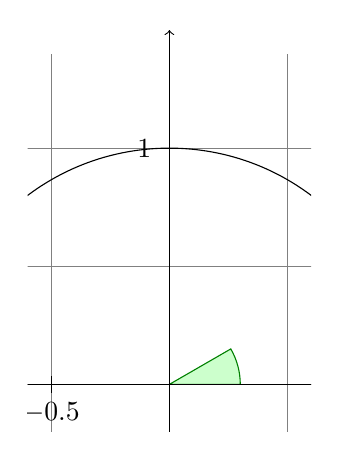
\begin{tikzpicture}[scale=3]
  \clip (-0.6,-0.2) rectangle (0.6,1.51);
  \draw[step = .5cm, help lines] (-1.4,-1.4) grid (1.4,1.4);
  \filldraw[fill=green!20,draw = green!50!black] (0,0) -- (3mm,0mm)
  arc [start angle = 0, end angle = 30,radius = 3mm] -- cycle;
  \draw[->] (-1.5,0) -- (1.5,0);
  \draw[->] (0,-1.5) -- (0,1.5);
  \draw (0,0) circle [radius=1cm];
  \foreach \x in {-1,-0.5,1}
  \draw(\x cm, 1pt) -- (\x cm, -1 pt) node [anchor = north] {$\x$};
  \foreach \y in {-1,-0.5,1}
  \draw(1pt,\y cm) -- (-1pt, \y cm) node[anchor = east] {$\y$};
\end{tikzpicture}
\end{lstlisting}

The generated figure is shown as:
\begin{center}
\includegraphics[width=0.5\textwidth]{/Users/chaolongzhang/Dropbox/mstemc_hugo/static/img/tikz/example4.pdf}
\end{center}


\section{Some Basic Rules in TikZ}
\label{sec:org171b856}


\begin{enumerate}
\item The options appear in \texttt{[]}. No matter it is an object or an operation, the
contents in the following  \texttt{[]} serve as options.

Options \texttt{[]} can be at the very beginning of the environment \texttt{tikzpicture}
following the operation, following the object.

\item \texttt{\textbackslash{}filldraw} is a good command. It draws a closed loop and fill it with color or
pattern. The colors for filling and drawing can be different.

\item Coordinates can be specified in x-y format, polar format.
\begin{itemize}
\item The easiest way is \texttt{(x,y)} which means \texttt{x} cm in the x-axis and \texttt{y} cm in the
y-axis;
\item \texttt{(a:x)} is the polar format which means \texttt{x} cm in direction \texttt{a} degree.
\end{itemize}
\item \texttt{(<p> |- <q>)} is another way to specify coordinates for example \texttt{(30:1 |- 0,0)}
which means the interaction of a vertical line through \texttt{(30:1)} and a
horizontal line through \texttt{(0,0)} .
\item Relative coordinates are possible with \texttt{+} and \texttt{++} in front of \texttt{(x,y)} and \texttt{(a:x)} .
\texttt{+} is relative to the closest coordinate whereas \texttt{++} is relative to the very
first coordinate of current path.
\end{enumerate}

\section{Some tips for in TikZ}
\label{sec:org46592f8}


\begin{enumerate}
\item To use \texttt{intersections} to specify a coordinate, you need to include the
library, i.e. \texttt{\textbackslash{}usetikzlibrary\{intersections\}} is a must.
\end{enumerate}


\lstset{language=C,label= ,caption= ,captionpos=b,firstnumber=1,numbers=left}
\begin{lstlisting}
int main()
{
  int i=0;
  printf();
}
\end{lstlisting}

\bibliography{../../research_library/zcl}
\bibliographystyle{unsrt}
\end{document}
